\documentclass[11pt, oneside]{article}   	% use "amsart" instead of "article" for AMSLaTeX format
\usepackage{geometry}                		% See geometry.pdf to learn the layout options. There are lots.
\geometry{letterpaper}                   		% ... or a4paper or a5paper or ... 
\usepackage{graphicx}				% Use pdf, png, jpg, or eps§ with pdflatex; use eps in DVI mode
								% TeX will automatically convert eps --> pdf in pdflatex		
\usepackage{amssymb}
\usepackage{amsmath}
\usepackage{parskip}
\usepackage{color}
\usepackage{hyperref}

\graphicspath{{/Users/telliott_admin/Dropbox/Tex/png/}}
% \begin{center} 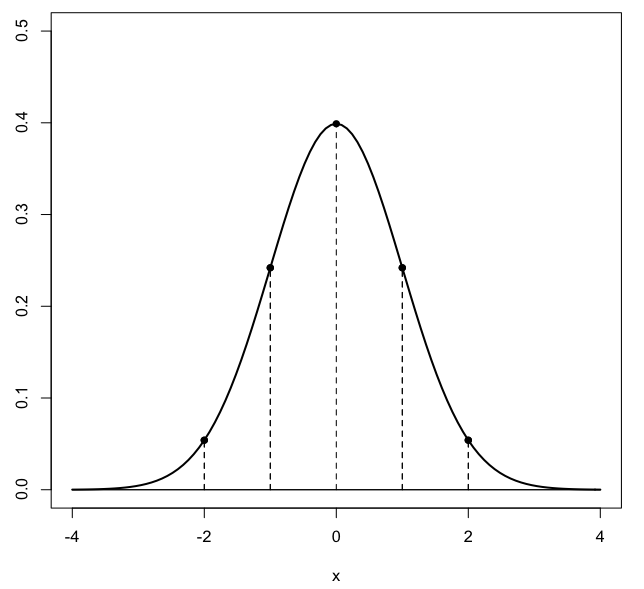
\includegraphics [scale=0.4] {gauss3.png} \end{center}

%break
\title{Riemann sums with graduated intervals}
\date{}

\begin{document}
\maketitle
\Large

\subsection*{intervals of unequal width}
Courant and John describe a variation on Riemann sums using intervals of unequal (but graduated) width.  This "trick" allows them to derive the formula for 
\[ \int x^n \ dx = \frac{x^{n+1}}{n+1} \]
\[ \int_a^b x^n \ dx = \frac{b^{n+1} - a^{n+1}}{n+1} \]
for all natural numbers $n$ first, and then with some elaborations, for real $n$ except $n = -1$.

\subsection*{Fermat version}
I also found a proof on the web, due to Fermat.  We'll look at that one first.

\url{http://fredrickey.info/hm/CalcNotes/Fermat-Integration.pdf}

It is really the basis for the Courant and John proof.  It achieves simplicity by using the interval $[0,b]$ with its lower bound at zero.

Let $E$ be a positive constant less than $1$.  Divide the region $[0,b]$ into subintervals with boundaries 
\[ \dots bE^3, bE^2, bE, b \]

How do we get the number of rectangles to increase to infinity?  By letting $E \rightarrow 1$ and taking the limit.

Construct rectangles in the usual way that circumscribe the curve $y = x^n$ and add up their areas.  For the $i$th rectangle, the width is
\[ bE^i - bE^{i+1} \]
($bE^{i+1} < bE^i$), and the height is
\[ (bE^i)^n \]
so the overall sum is
\[ S = \sum_{i = 0}^{\infty} (bE^i)^n \ (bE^i - bE^{i+1}) \]
\[ = b^{n+1} \sum_{i = 0}^{\infty} (E^i)^n \ (E^i - E^{i+1}) \]
\[ = b^{n+1} \sum_{i = 0}^{\infty} (E^i)^{n+1} \ (1 - E) \]
\[ = b^{n+1} \ (1 - E) \ \sum_{i = 0}^{\infty} (E^{n+1})^i \]

Since $E$ is a positive constant less than $1$, $E^{n+1}$ is also.  Let $q = E^{n+1}$.  The sum becomes
\[ \sum_{i = 0}^{\infty} q^i = q^0 + q^1 + q^2 + q^3 + \dots \]
Recall that
\[ \frac{1}{1-x} = 1 + x + x^2 + x^3 + \dots \]
for $|x| < 1$.  

So, going back to $E$ we have
\[ S = b^{n+1} \ (1 - E) \ \frac{1}{1 - E^{n+1}} \]
and using the same identity again
\[ 1 - x = \frac{1}{1 + x + x^2 + x^3 + \dots } \]
so
\[ S = b^{n+1} \ \frac{1}{(1 + E + E^2 + E^3 + \dots)(1 - E^{n+1})} \]
All the terms in the infinite series starting at $E^{n+1}$ acquire counterparts with a minus sign, hence
\[ = b^{n+1} \ \frac{1}{1 + E + E^2 + E^3 + \dots + E^n} \]

Now take the limit as $E \rightarrow 1$.  The fraction becomes just
\[ \frac{1}{1 + E + E^2 + E^3 + \dots + E^n}  = \frac{1}{n+1} \]
and we have
\[ \int_0^b x^n = \frac{b^{n+1}}{n+1} \]
which is what we get when we evaluate $x^{n+1}$ on the interval $[0,b]$ and then divide by $n+1$.

\subsection*{Courant version}
The more rigorous approach follows.

\begin{center} 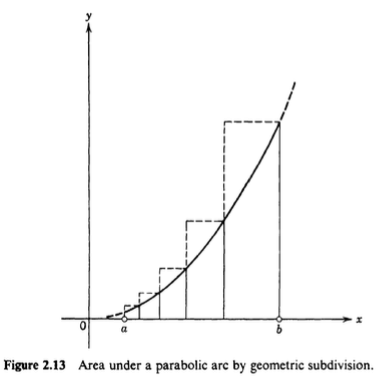
\includegraphics [scale=0.6] {Courant_2_13.png} \end{center}
We subdivide the interval $[a, b]$ by points with spacing that increases by a factor of $q$ at each step
\[ a,\ aq,\ aq^2,\ \dots \ aq^{n-1},\ aq^n \]

At the final, nth step we have 
\[ aq^n = b \]
Solving for the common ratio $q$ we have
\[ q = (b/a)^{1/n} \]
The points of division are
\[ x_i = aq^i \]
The width of the $i$th rectangle is
\[ \Delta x_i = aq^i - aq^{i-1} = aq^i \ (1 - \frac{1}{q}) \]
\[= aq^i \ [ \ \frac{q-1}{q} \ ] \]
The widest rectangle is the last one
\[ \Delta x_n = aq^n \ [ \ \frac{q-1}{q} \ ] \]
\[ = b \ [ \ \frac{q-1}{q} \ ] \]
In the usual way, we will let the number of rectangles $n \rightarrow \infty$.  

At the same time, since
\[ q = (b/a)^{1/n} \]
then $q \rightarrow 1$.  

So then $\Delta x_n \rightarrow 0$, and so do all the other rectangles, which are smaller.

The function of interest is to raise $x$ to the positive integer power $p$.  For each rectangle, the area is
\[ A_i = x_i^p \ \Delta x_i \]
\[ = (aq^i)^p \ aq^i \ [ \ \frac{q-1}{q} \ ] \]
\[ = a^{p+1} \ (q^i)^{p+1}\ [ \ \frac{q-1}{q} \ ] \]
\[ = a^{p+1} \ (q^{p+1})^i \ [ \ \frac{q-1}{q} \ ] \]

For the integral, we need to add all these up (from $i = 1$ to $i = n$):
\[ I = \sum_{i=1}^n a^{p+1} \ (q^{p+1})^i \ [ \ \frac{q-1}{q} \ ] \]
We can take out values that don't depend on $i$ from the summation:
\[ I = a^{p+1} \  [ \ \frac{q-1}{q} \ ] \  \sum_{i=1}^n  (q^{p+1})^i  \]

Recall that for a geometric series with common ratio $r$ the nth sum (starting from $i=0$) is
\[ S_n = 1 + r + r^2 \dots + r^n =  \sum_{i=0}^n r^i \]
\[ = \frac{1 - r^n}{1 - r} = \frac{r^n - 1}{r - 1}  \]
Substituting $q$ for $r$:
\[ S_n = \frac{q^n - 1}{q - 1}  \]

For the expression above
\[  \sum_{i=1}^n  (q^{p+1})^i  \]
we factor out one $q^{p+1}$ so as to start from $i=0$
\[ = q^{p+1} \ \sum_{i=0}^n  (q^{p+1})^i  \]
and then the common ratio is $q^{p+1}$ and the sum is
\[ \sum_{i=0}^n  (q^{p+1})^i = \frac{(q^{p+1})^{n} - 1}{q^{p+1} - 1} = \frac{q^{n(p+1)} - 1}{q^{p+1} - 1} \]

The whole sum or integral $I$ that we seek is
\[ I = a^{p+1} \  [ \ \frac{q-1}{q} \ ] \  q^{p+1} \ \frac{q^{n(p+1)} - 1}{q^{p+1} - 1} \]
\[ = a^{p+1} \ (q-1) \ q^p  \ \frac{q^{n(p+1)} - 1}{q^{p+1} - 1} \]
\[ = a^{p+1} \  (q-1) \ q^p  \ \frac{(b/a)^{p+1} - 1}{q^{p+1} - 1} \]
Since
\[ a^{p+1} \ [ \ (b/a)^{p+1} - 1 \ ] \ = b^{p+1} - a^{p+1} \]
we obtain
\[ I = \ [ \ b^{p+1} - a^{p+1} \ ] \ q^p \ \frac{q-1}{q^{p+1} - 1} \]

Referring to the sum for a geometric progression again, we have from above 
\[ S_n = \frac{q^n - 1}{q - 1}  \]
So (for $q \ne 1$) and $n=p+1$, the inverse of that is what we have for the right-hand term
\[ \frac{q-1}{q^{p+1} - 1} = \frac{1}{S_{p+1} }  \]
where
\[ S_{p+1} = 1 + q + q^2 + \dots + q^{p+1} \]
Substituting
\[ I = \ [ \ b^{p+1} - a^{p+1} \ ] \ q^p \ \frac{1}{1 + q + q^2 + \dots + q^{p+1}}  \]

As we saw near the beginning, as $n \rightarrow \infty$, $q \rightarrow 1$, and so do all the powers of $q$ so the term
\[ q^p = 1 \]
and also
\[ 1 + q + q^2 + \dots + q^{p+1} = p + 1 \]
so the fraction is just equal to $1/(p+1)$ and we have finally:
\[ I = \ [ \ b^{p+1} - a^{p+1} \ ] \ \frac{1}{p + 1} \]
which is what we sought to prove.

If you look carefully at this proof, you'll see that it follows Fermat exactly, but is more general by including $a$ as the lower bound.

\end{document}